Ahora, con la desviación estandar debida a la posición de la fibra en el dispositivo experimental determianda, procedemos a llevar a cabo un estudio donde intervenga únicamente otra incertidumbre adicional, la debida a la preparación de cada una de las fibras utilizas.

Esta surje debido al hecho de que cada una de las fibras necesita de un proceso de preparación antes de poder estar ópticamente preparada para medir. Este proceso, como ya se ha comentado, incluye cortes con una guillotina especialmente diseñada en los talleres del IFIC, puido de las fibras con lijas de distinto grosor, limpieza de la superficie, etc. En resumen, se trata de un método individual para cada fibra que puede presentar cierta dispersión.

El estudio consistirá en preparar 10 muestras de $200~\mm$ diferentes para cada tipo de fibra y realizar la medida, con ayuda del picoamperímetro, de la intensidad promedio $I_i$ y su error para un conjunto de 100 medidas para cada una de estas fibras. Además, dado que solo pretendemos tomar una única medida en cada fibra, se realizará la medida para cuatro intensidades de alimentación de la LED diferentes, $0.05$, $0.1$, $0.15$ y $0.2~\milli\ampere$. De esta forma comprobaremos el correcto funcionamiento del sistema para cada uno de los casos al obtener una dependencia lineal.

El resultado de este experimento se representa en las figuras \ref{medidasnoclad}, \ref{medidassingleclad} y \ref{medidasmulticlad} 

\begin{figure}[hbtp]
\centering
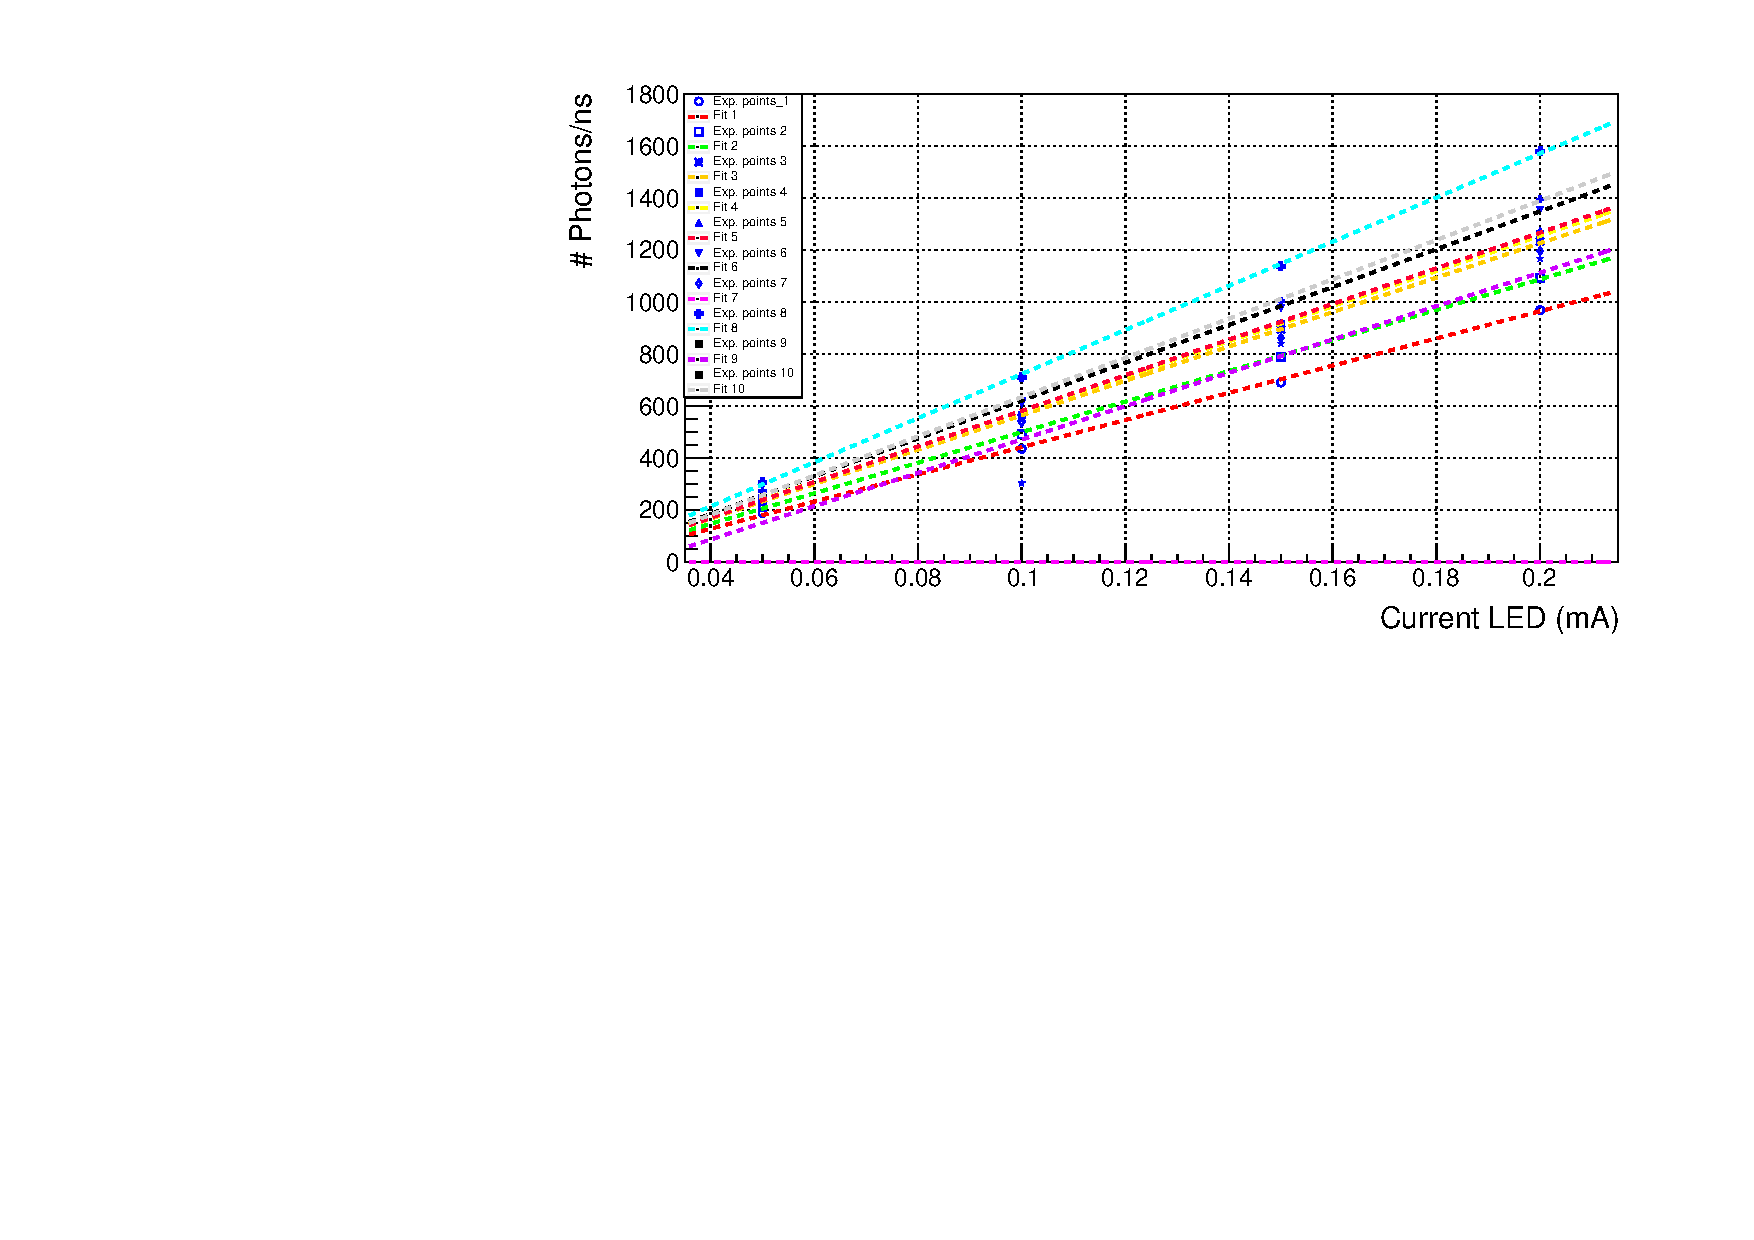
\includegraphics[scale=0.7]{Figuras/SamplesNoClad.pdf}
\caption{Intensidad obtenida en 10 muestras diferentes de fibras no clad de $200~\mm$ frente a la alimentaicón de la LED\label{medidasnoclad}}
\end{figure}

\begin{figure}[hbtp]
\centering
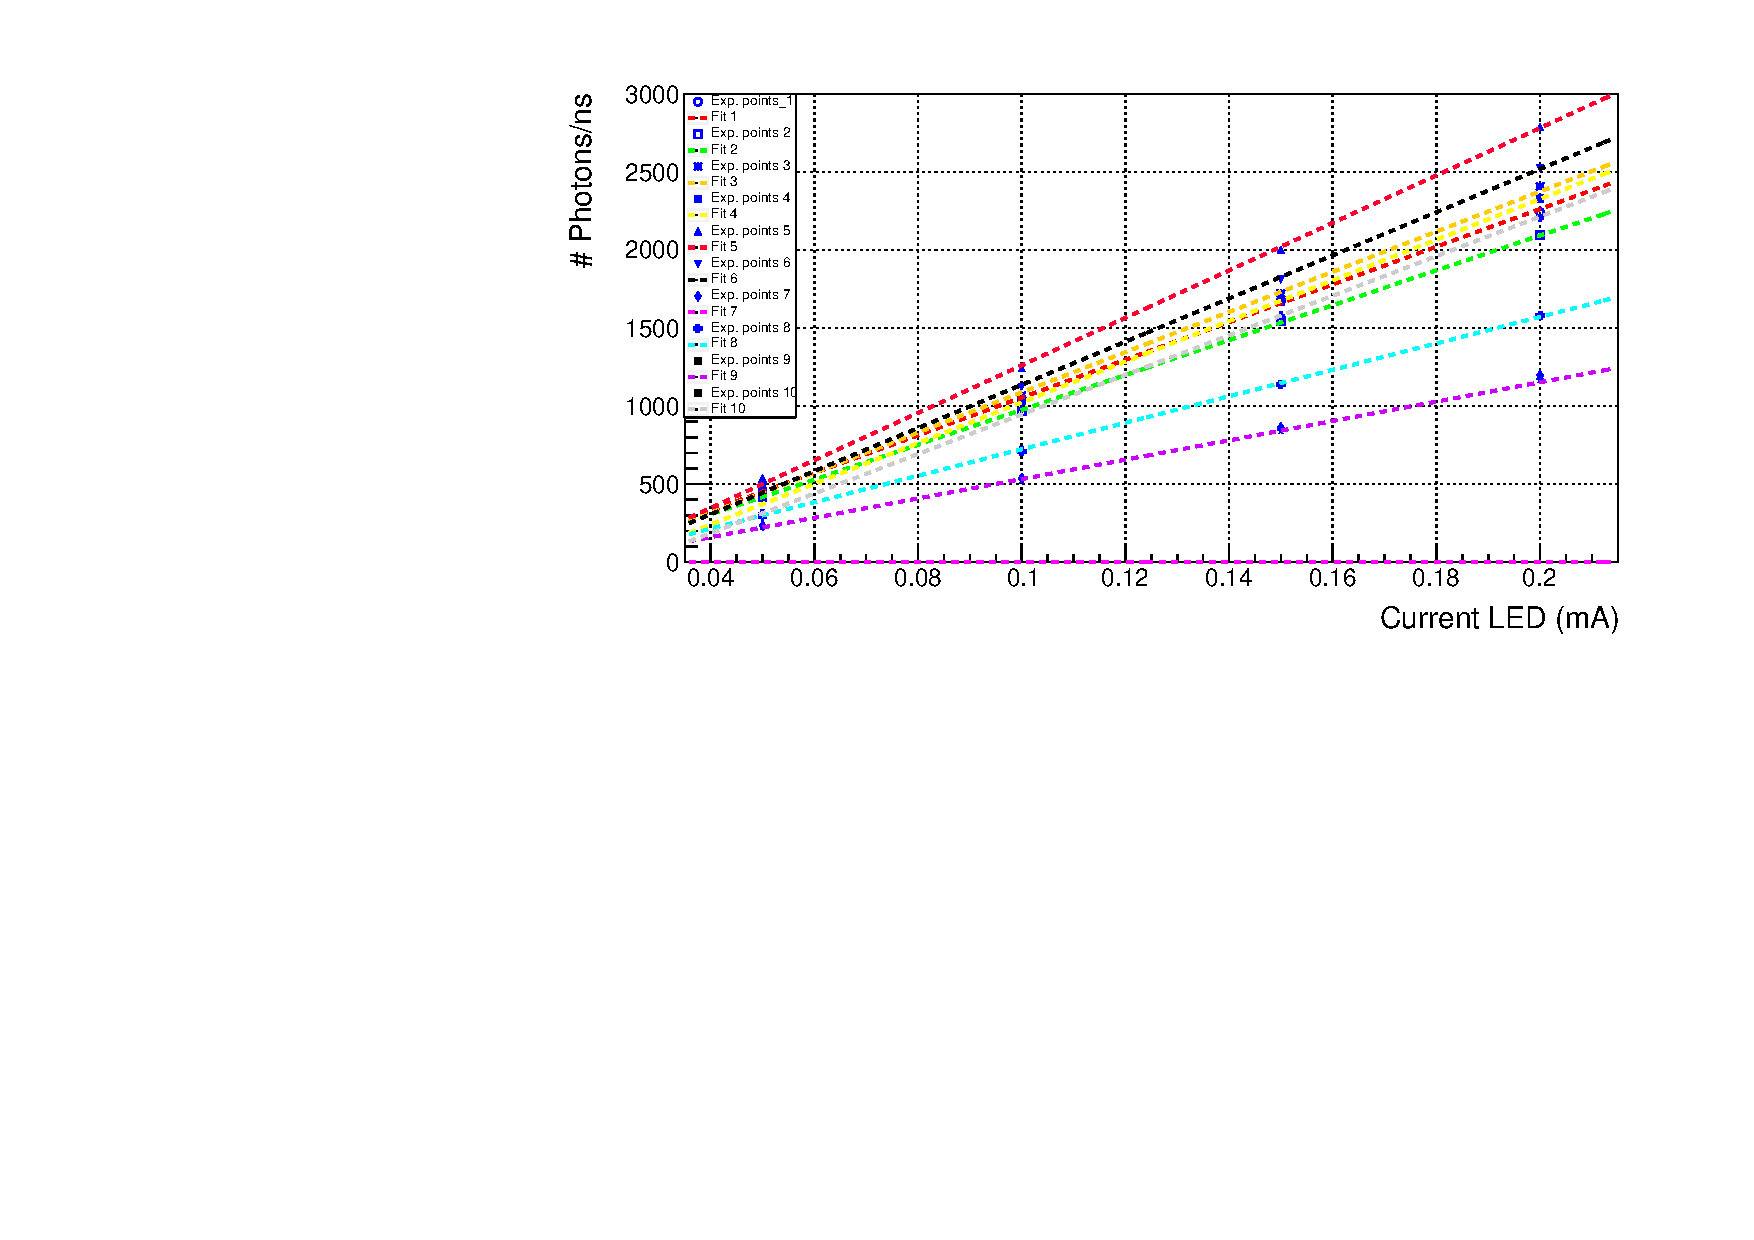
\includegraphics[scale=0.7]{Figuras/SamplesSingleCladHouda.pdf}
\caption{Intensidad obtenida en 10 muestras diferentes de fibras single clad de $200~\mm$ frente a la alimentaicón de la LED\label{medidassingleclad}}
\end{figure}

\begin{figure}[hbtp]
\centering
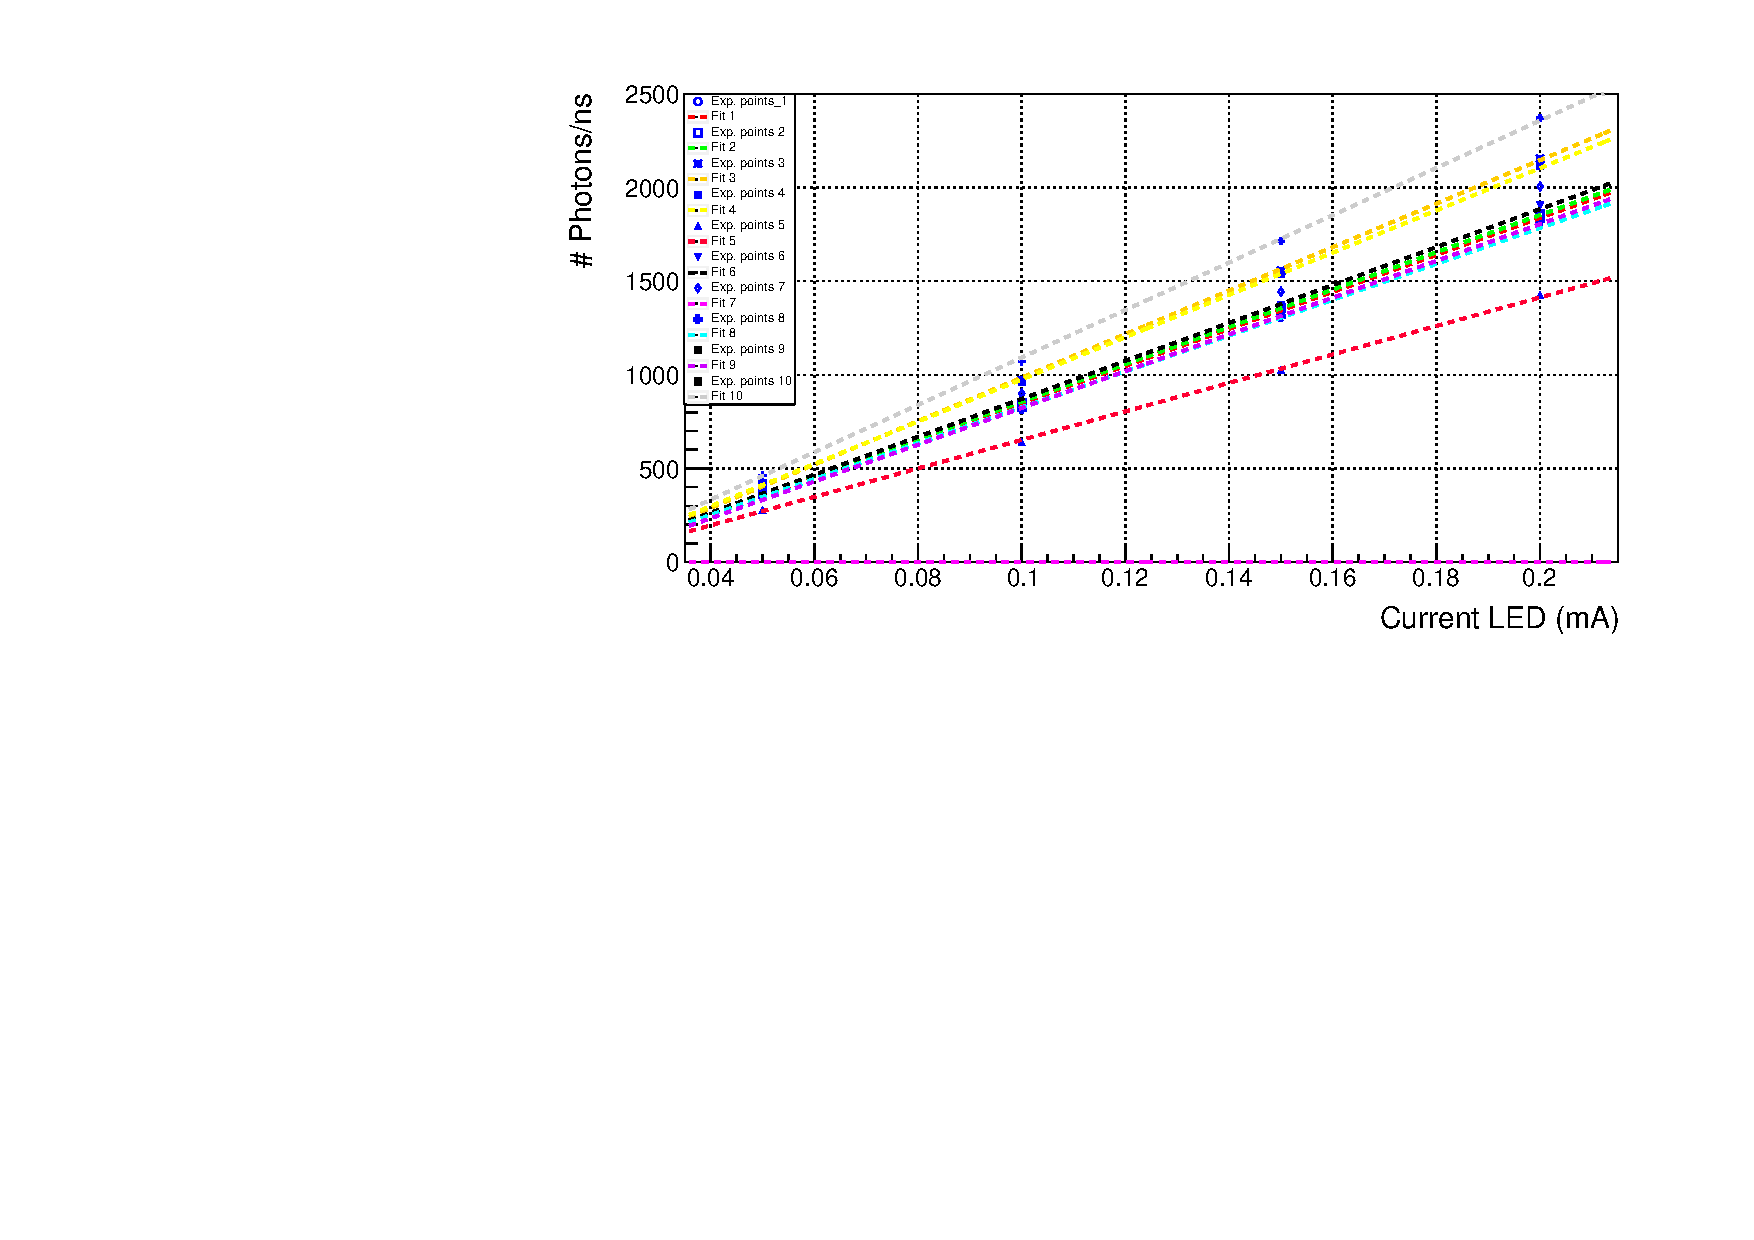
\includegraphics[scale=0.7]{Figuras/SamplesMultiClad.pdf}
\caption{Intensidad obtenida en 10 muestras diferentes de fibras multi clad de $200~\mm$ frente a la alimentaicón de la LED\label{medidasmulticlad}}
\end{figure}

En este podemos apreciar esta perfecta linealidad existente entre la señal y la alimentación de la LED para cada una de las muestras. También podemos observar que, efectivamente, existen diferencias entre la señal obtenidas con diferentes muestras de un mismot tipo de fibra. Ello es debido a dos razones, a la posición de la fibra en el dispostivo experimental y al proceso de preparación de la fibra. Por tanto, la desviación estandar total calculada en este experimento será la suma cuadrática de ambas según se expresa en la ecuación \ref{incertidumbreint}.

Con ayuda de las ecuaciones \ref{ecuacionmedia} y \ref{ecuaciondesviacionestandar}, obtenemos ahora el promedio de las diez medidas y la desviación estandar de estas para cada alimentación de la LED utilizada y cada tipo de fibra. El resultado puede verse en la tabla \ref{senalydesviacion}.

\begin{table}[H]
\begin{center}
\begin{tabular}{l | c | c | c | c }
Intensidad LED $(\milli\ampere)$ &  No Clad $(N.\gamma~/\nano\second)$ & Single Clad $(N.\gamma~/\nano\second)$ & Multi Clad $(N.\gamma~/\nano\second)$ \\
\hline \hline
$0.05$ & $243.46 \pm 9.82$ & $383.81 \pm 33.23$ & $376.676 \pm 14.96$\\ 
$0.1$ & $540.62 \pm 33.51$ & $922.68 \pm 73.97$ & $870.87 \pm 34.48$\\
$0.15$ & $902.74 \pm 36.83$ & $1485.10 \pm 119.90$ & $1396.60 \pm 55.24$\\
$0.2$ & $1252.62 \pm 50.48$ & $2053.78 \pm 166.391$ & $1932.57 \pm 76.02$\\

\end{tabular}
\caption{Señal y desviación estandar asociada a cada tipo de fibra y para cada alimetnación de la LED\label{senalydesviacion}}
\end{center}
\end{table}

Vemos que añadir un clad a la fibra produce una mejora considerable en la eficiencia de colección de luz. Sin embargo, para las distancias empleadas en el experimento, $200~\mm$, la mejora producida al añadir un segundo clad es inferior a las perdidas producidas por el hecho de tener que reducir el nucleo para ello, es decir, obtenemos una señal menor al aumentar el grosor del clad. Seguramente al aumentar de forma considerable la longitud de la fibra llegará un punto en el que esta situación cambie y la mejora producida por el doble clad sea superior a las perdidas producidas por la reducción del nucleo. Este sería un punto interesante y que se someterá a estudio en un futuro.

Hay que tener en cuenta que la señal obtenidas para el caso de fibras single clad esta en conflicto con la obtenidos en el apartado anterior. Tomaremos este valor como más fiable debido al hecho que este surje como promedio de 10 muestras distitnas de fibras mientras que el estudio anterior se ha realizado en todo momento sobre una misma muestra.

Ahora representamos estas tres dependencias promedidas en la figura \ref{mediafibras}:

\begin{figure}[H]
\centering
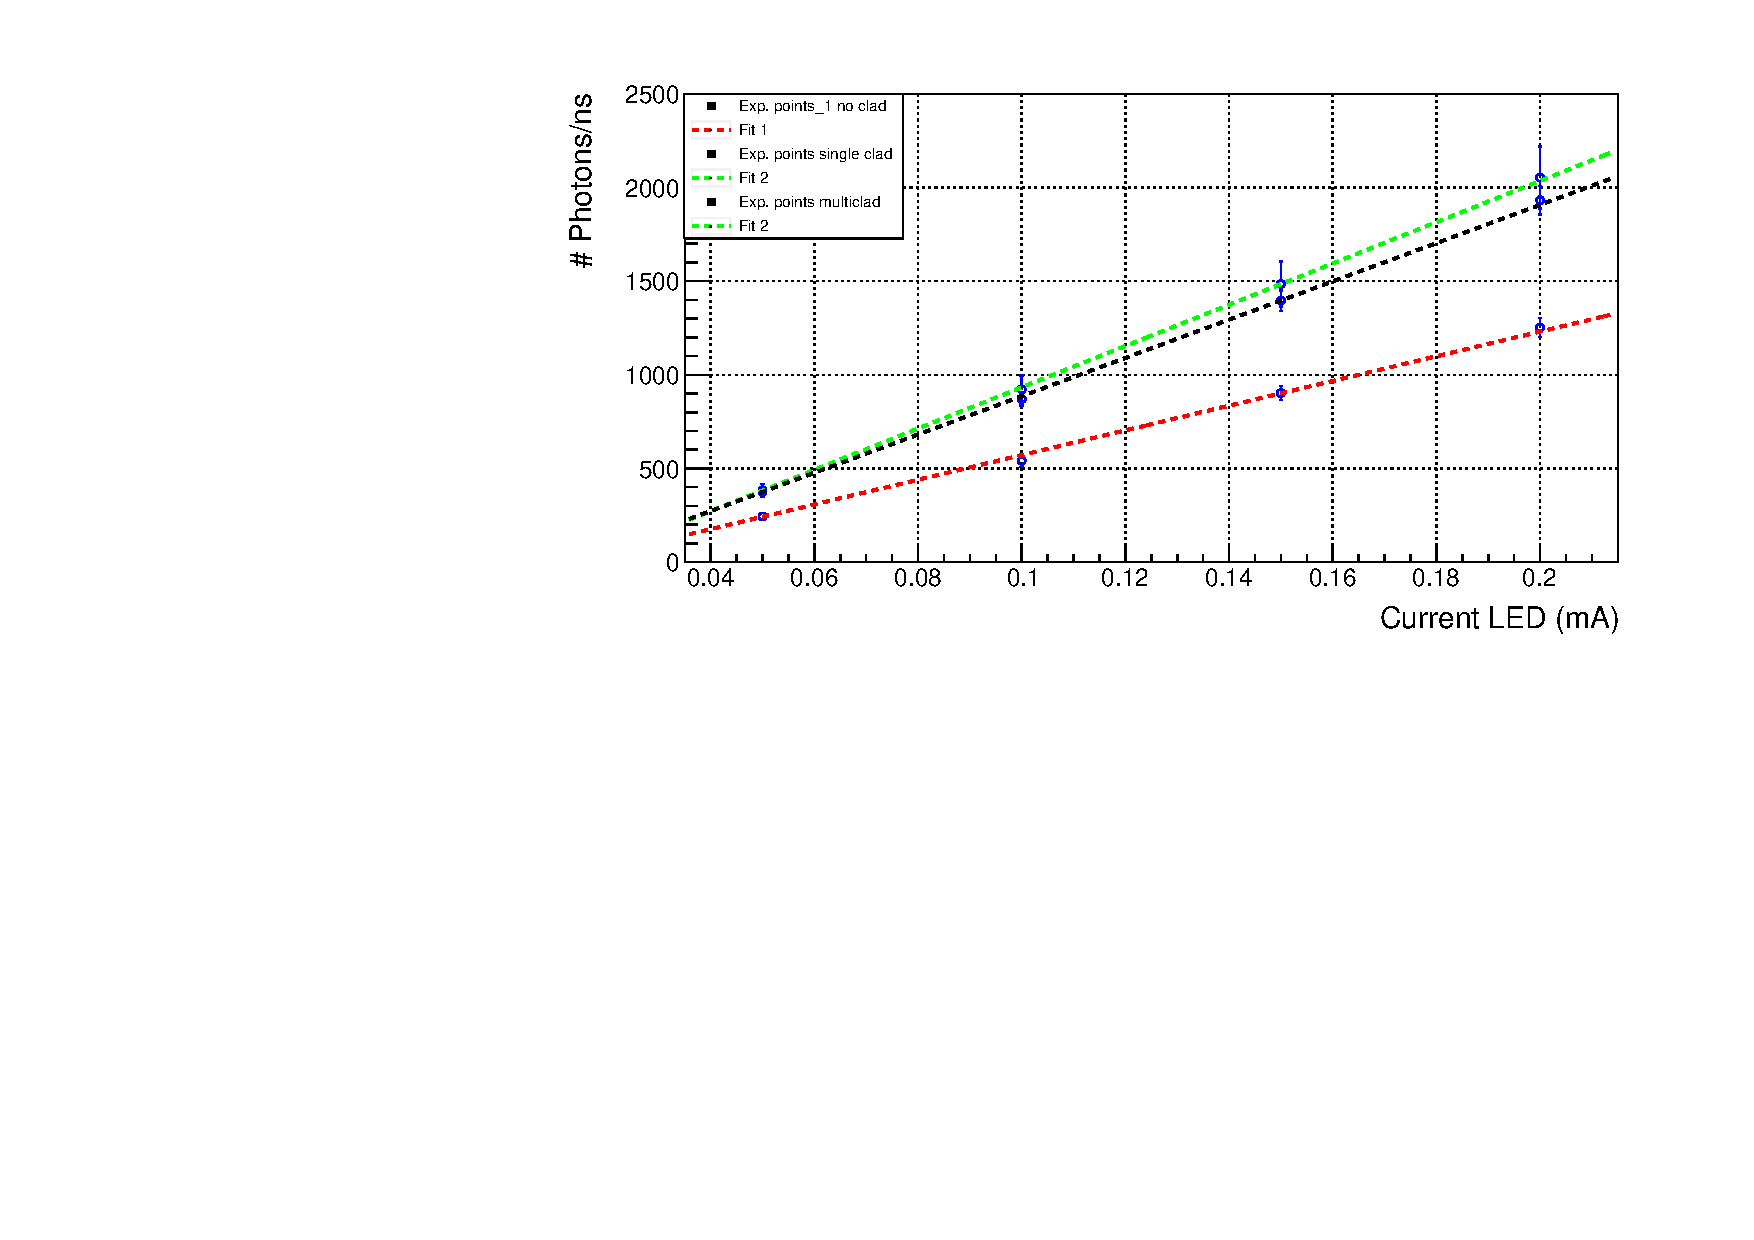
\includegraphics[scale=0.7]{Figuras/HoudaCase.pdf}
\caption{Media y desviación estandar de las 10 muestras de fibras de cada tipo de $200~\mm$ frente a la alimentaicón de la LED\label{mediafibras}}
\end{figure}


Además de lo comentado anteriormente, podemos observar una relación perfecta mente lineal para cada uno de los tipos lo cual nos permite verificar que el estudio se ha realizado adecuadamente.

Finalmente obtenemos la dispersión estandar relativa como el cociente entre la dispersión estandar y la señal. Realizamos este para cada una de las cuatro intensidades de alimentación de la LED y, dado que teóricamente este debería de ser constante, obtenemos el promedio. Los resultados pueden observarse en la tabla \ref{relativefibers}:

\begin{table}[H]
\begin{center}
\begin{tabular}{l | c | c | c | c }

Intensidad LED $(\milli\ampere)$ & D. S. R. (No Clad) & D. S. R. (Single Clad) & D. S. R. (Multi Clad)\\
\hline \hline
0.05 & $4.03$ & $8.66$ & $3.97$\\ 
0.1 & $6.20$ & $8.02$ & $3.91$\\
0.15 & $4.08$ & $8.04$ & $3.96$\\
0.2 & $4.03$ & $8.10$ & $3.93$\\
\hline \hline
Averege & $4.59\pm 0.54$ & $8.21\pm0.15$ & $3.96 \pm 0.01$

\end{tabular}
\caption{Desviación estandar relativa asociada a cada tipo de fibra y para cada alimetnación de la LED\label{relativefibers}}
\end{center}
\end{table}

Estos valores corresponden a la desviación estandar relativa total para cada una de las tres fibras. Ahora, con ayuda de la ecuación \ref{incertidumbreint}, es inmediato obtener el valor de la incertidumbre relativa asociada al proceso de fabricación. Un resumen de esto se muestra en la tabla \ref{incertidumbres}

\begin{table}[H]
\begin{center}
\begin{tabular}{l | c | c | c | c }
Type of fiber & $\sigma_{total,rel}$ (\%) & $\sigma_{pos,rel}$ (\%) &$\sigma_{int,rel}$ (\%)\\
\hline \hline
No Clad & 4.58 +- 0.53 & 3.37 & 3.10\\ 
Single Clad & 8.21 +- 0.15 & 2.17 & 7.92\\
Multi Clad & 3.96 +- 0.01 & 1.04 & 3.82
\end{tabular}
\caption{Resumen de las incertidumbres obtenidas en el estudio de las fibras\label{incertidumbres}}
\end{center}
\end{table}

Podemos observar que, la mínima incertidumbre en el proceso de preparación de la fibra se encuentra en la fibra sin clad, es decir, el elemento de la fibra más resistente a este proceso es el nucleo. Podemos observar que, al añadirle un clad simple esta incertidumbre se dispara. El motivo de ello es que el clad, por el hecho de ser tan fino, se estropea con facilidad en el proceso de preparación, un proceso relativamente agresivo, algo que puede llegarse a observar incluso a simple vista. Sin embargo, podemos observar que, el hecho de añadir un segundo clad mejora notablemente la incertidumbre. Es decir, este segundo clad no solo aporta una lijera mejora en al eficiencia de colección de luz, si no que aporta una mayor robustez a la fibra. 